\chapter{Getting Started} \label{ch:gettingStarted}

\section{Installation} \label{sec:installation}

\vvase{} does not include any installation process or changes to the machine registry.  Simply place the executable and the pdf manual into the same directory.  After running the first time, any changes to the default settings are saved to a configuration file which will appear in the directory from which the application is run.

\section{Overview} \label{sec:overview}

Upon starting \vvase{} for the first time, the screen will look like Fig.~\ref{fig:defaultStartup}.  Counter-clockwise from the top left corner of the window are the Systems Tree \(\S~\ref{ssec:systemsTree}\), Edit Panel \(\S~\ref{ssec:editPanel}\), Output Pane \(\S~\ref{ssec:outputPane}\), Output List \(\S~\ref{ssec:outputList}\) and Main Display Area \(\S~\ref{ssec:mainDisplayArea}\).  Above these elements are two toolbars, the Kinematics Toolbar \(\S~\ref{ssec:kinematicsToolbar}\) and the 3D Toolbar \(\S~\ref{ssec:3DToolbar}\).  Across the top of the window is a typical menu bar, the contents of which are described in \S~\ref{ssec:menu}.  All of these elements can be dragged, floated or docked to create the desired layout.

\begin{figure}
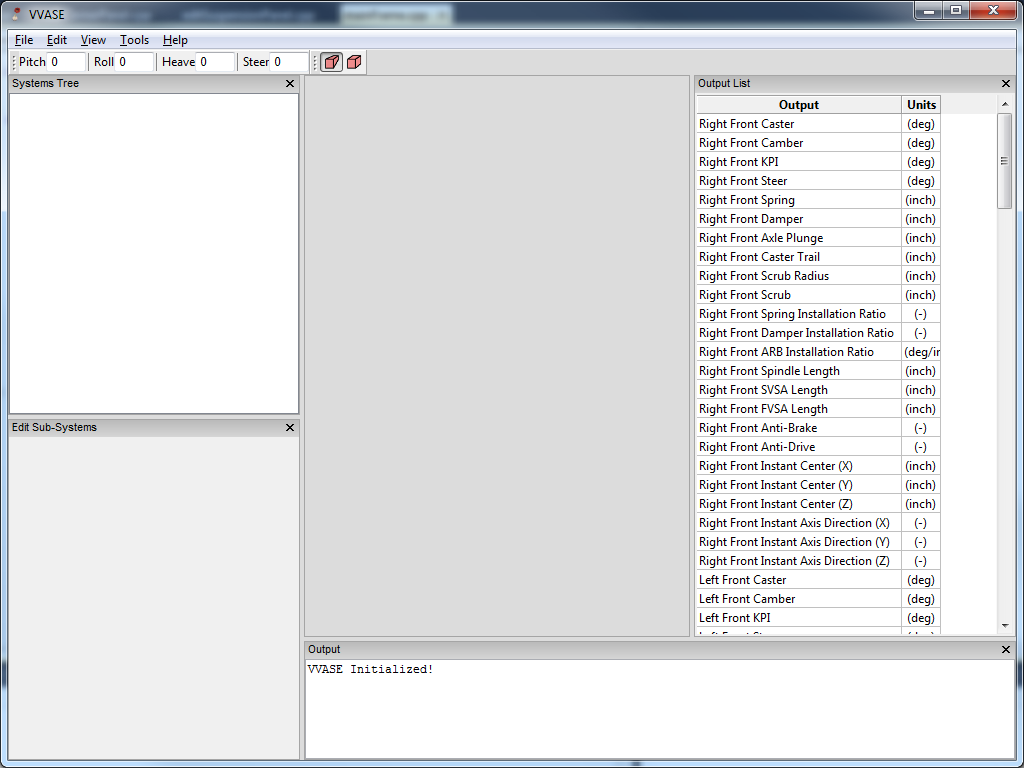
\includegraphics[width=\textwidth]{images/defaultStartup} \label{fig:defaultStartup}
\caption{Default screen configuration}
\centering
\end{figure}

\subsection{Systems Tree} \label{ssec:systemsTree}

The Systems Tree lists all of the files that are currently open.  Some files include sub-items which can be accessed by expanding the parent item.  Right-clicking on Systems Tree entries results in a context menu from which files can be closed.

%% TODO:  What else is in context menu

\subsection{Edit Panel} \label{ssec:editPanel}

The Edit Panel is where the core modifications to all files are made.  When a file is selected by either selecting its tab in the Main Display Area or clicking on it in the Systems Tree, the Edit Panel changes to show options relevant to the selected file.  For files that include sub-items in the Systems Tree, each sub-item may have different editable parameters.

\subsection{Output Pane} \label{ssec:outputPane}



\subsection{Output List} \label{ssec:outputList}



\subsection{Main Display Area} \label{ssec:mainDisplayArea}



\subsection{Kinematics Toolbar} \label{ssec:kinematicsToolbar}



\subsection{3D Toolbar} \label{ssec:3DToolbar}



\subsection{Menu Bar} \label{ssec:menuBar}



\section{Options} \label{sec:options}

In additon to display customization, there are several ways in which the behavior of \vvase{} can be adjusted to suit user preferences.

\begin{figure}
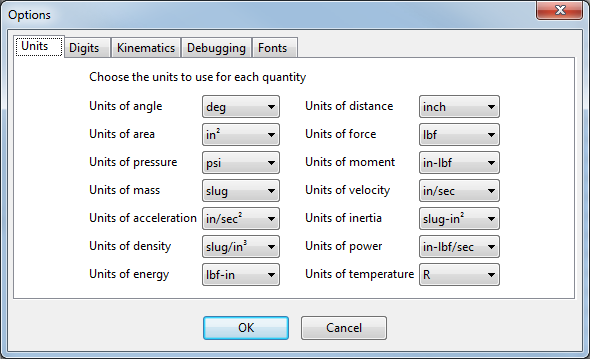
\includegraphics[width=\textwidth]{images/optionsUnits} \label{fig:optionsUnits}
\caption{Units options}
\centering
\end{figure}

\begin{figure}
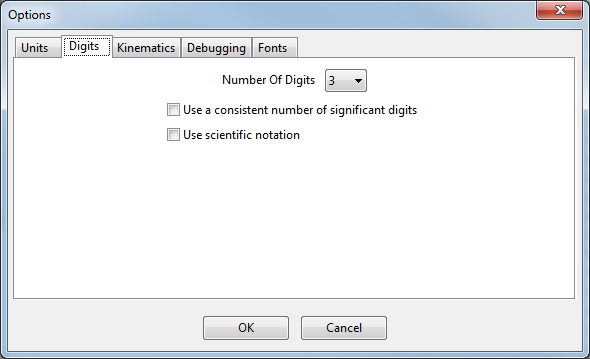
\includegraphics[width=\textwidth]{images/optionsDigits} \label{fig:optionsDigits}
\caption{Digits options}
\centering
\end{figure}

\begin{figure}
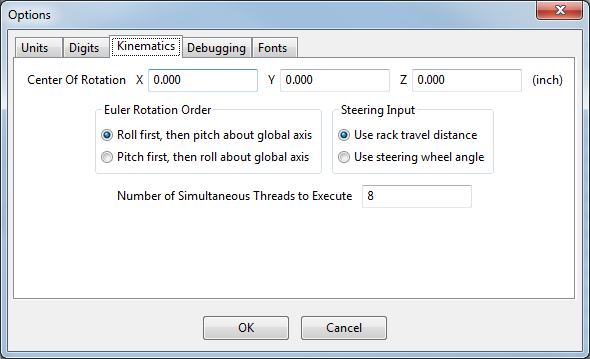
\includegraphics[width=\textwidth]{images/optionsKinematics} \label{fig:optionsKinematics}
\caption{Kinematics options}
\centering
\end{figure}

\begin{figure}
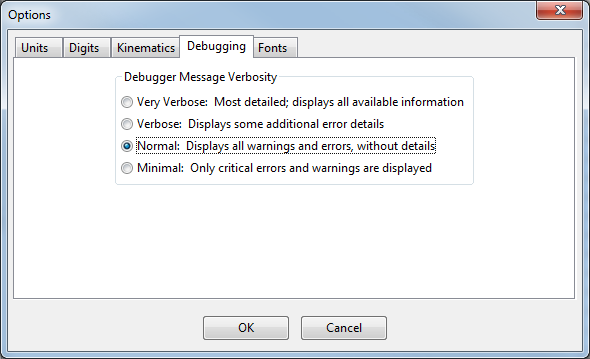
\includegraphics[width=\textwidth]{images/optionsDebugging} \label{fig:optionsDebugging}
\caption{Debugging options}
\centering
\end{figure}

\begin{figure}
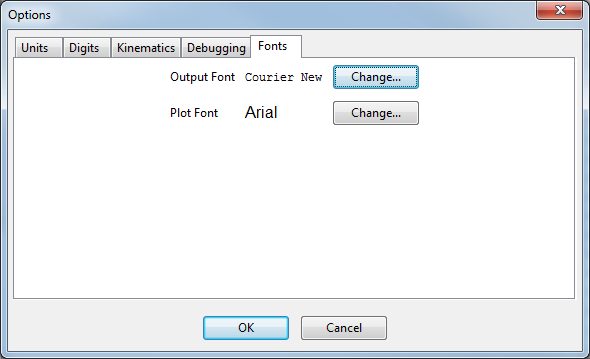
\includegraphics[width=\textwidth]{images/optionsFonts} \label{fig:optionsFonts}
\caption{Fonts options}
\centering
\end{figure}
